\documentclass{beamer}    % 14pt je nenujen
\usepackage[T1]{fontenc}
\usepackage[utf8]{inputenc}
\usepackage[slovene]{babel}
\usepackage{pgfpages}           % privat zapiski
\usepackage{amsfonts}
\usepackage{amsmath,amsthm}     % pravilen izpis v "math mode"
%\usepackage{hyperref}
\usepackage{graphicx}           % za slike
\usepackage{tikz}
\usepackage{multicol}
\usepackage{ulem}
\usepackage{bibentry}
\usepackage{caption}
\usepackage{subcaption}

%\hypersetup{hidelinks}

\setbeamertemplate{theorems}[ams style]             % numbered da brez bold 

\setbeameroption{hide notes}                        % samo prosojnice
%\setbeameroption{show only notes}                   % samo zapiski
%\setbeameroption{show notes on second screen=right}  % oboje

\usepackage{palatino}
\usefonttheme{serif}

%\usecolortheme{beetle} %ali beetle morda ali seagull 

\setbeamertemplate{navigation symbols}{} % izklop navigacije
\setbeamertemplate{footline}[frame number]{} % oštevilčenje
\setbeamertemplate{note page}{\pagecolor{yellow!5}\insertnote}

\newtheorem{izrek}{Izrek}
\newtheorem{trditev}[izrek]{Trditev}
\newtheorem{posledica}[izrek]{Posledica}
\newtheorem{definicija}[izrek]{Definicija}
\newtheorem{naloga}[izrek]{Naloga}
\newtheorem{resitev}[izrek]{Naloga}

\author{Tim Kalan \\ \medskip
        \footnotesize Mentor: doc.~dr. Tilen Marc}
% \author{Tim Kalan}
% \institute[FMF]{Fakulteta za matematiko in fiziko}
% \title{
%     Kako se skupina podpiše? \\ 
%     \large (angl. \textit{How can a group sign?})}
\title{Kako se skupina podpiše?}
\date{27. maj 2024} 

\begin{document}

\begin{frame}
    \titlepage
\end{frame}

\begin{frame}
    \frametitle{Zakaj potrebujemo podpise?}
    \begin{itemize}
        \item Mislim, da si lahko predstavljate ... 
        \item Avtentikacija, integriteta
        \item Bančništvo, e-pošta, \texttt{ssh}, ...
    \end{itemize}
\end{frame}

\begin{frame}
    \frametitle{Kaj je podpis?}
    \begin{multicols*}{2}
        \textbf{Ročni podpis}
        \begin{itemize}
            \item Vsakič (približno) enak
            \item Enostavno ponarediti
            \item Težko (zares) preveriti
        \end{itemize}
        \columnbreak

        \textbf{Digitalni podpis}
        \begin{itemize}
            \item Vsakič unikaten
            \item Težko ponarediti
            \item Enostavno preveriti
        \end{itemize}
    \end{multicols*}
\end{frame}

\begin{frame}
    \frametitle{Kriptografija javnega ključa 1}
    \begin{figure}
        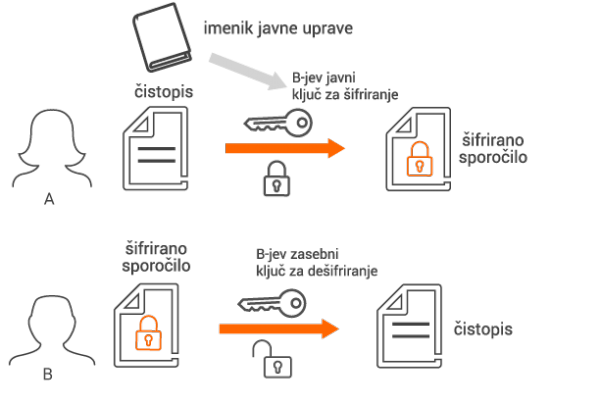
\includegraphics[width=\textwidth]{images/enkripcija.png}
    \end{figure}
\end{frame}

\begin{frame}
    \frametitle{Kriptografija javnega ključa 2}
    \begin{figure}
        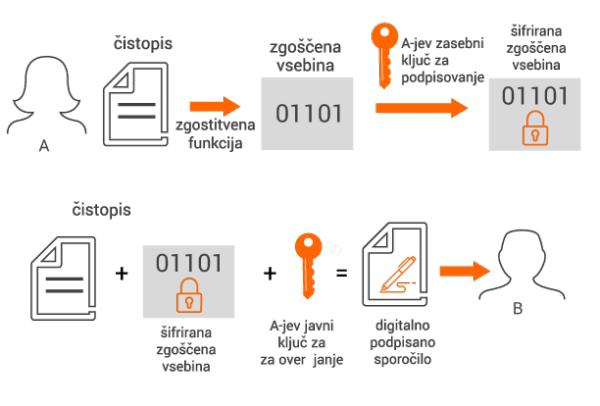
\includegraphics[width=\textwidth]{images/podpisovanje.png}
    \end{figure}
\end{frame}

\begin{frame}
    \frametitle{Zgostitvene funkcije}
    \begin{itemize}
        \item Psevdonaključne funkcije
        \item Enosmerne
        \item ">Enostavno"< izračunljive
    \end{itemize}
    \begin{align*}
        &\texttt{SHA-256(Ljubljana)} = \\
        &\texttt{b7f147d8b4a6703a951336654355071f} \\ 
        &\texttt{9752385f85d0860379e99b484aee7a82} \\
        &\texttt{SHA-256(Ljubljena)} = \\
        &\texttt{995d2d8ffb40e1838219e65dd2c66570} \\
        &\texttt{1ba34a90e11f7195a4b791838b6787fe} \\ 
    \end{align*}
    \begin{itemize}
        \item Naključni oraklji
    \end{itemize}
\end{frame}

\begin{frame}
    \frametitle{Primer digitalnega podpisa: RSA}
    Odličen primer za spoznavanje osnovnih konceptov:
    \vspace{1cm}
    \begin{itemize}
        \item Generiranje ključev
        \item Podpisovanje
        \item Preverjanje 
    \end{itemize}
\end{frame}

\begin{frame}
    \frametitle{RSA}
    \framesubtitle{Generiranje ključev}
    \begin{itemize}
        \item Izberemo dve \alert{veliki} praštevili $p$ in $q$ (kako?)
        \item Izračunamo $n = pq$ in $\phi(n) = (p-1)(q-1)$
        \item Izberemo $e$ tako, da je $1 < e < \phi(n)$ in $\gcd(e, \phi(n)) = 1$
        \item Izračunamo $d$ tako, da je $ed \equiv 1 \pmod{\phi(n)}$
    \end{itemize}
    \vspace{1cm}
    \begin{multicols*}{2}
        \textbf{Javni ključ}: $(n, e)$
        \columnbreak

        \textbf{Zasebni ključ}: $d (+ p, q)$
    \end{multicols*}
\end{frame}

\begin{frame}
    \frametitle{RSA}
    \framesubtitle{Podpisovanje in preverjanje}
    \begin{itemize}
        \item Sporočilo $m$ podpišemo tako, da izračunamo $s = m^d \bmod n$
        \item Podpis je par $(m, s)$
    \end{itemize}
    
    \vspace{1cm}
    \begin{itemize}
        \item Preverimo tako, da izračunamo $m' = s^e \bmod n$
        \item Podpis je pravilen, če je $m' = m$
    \end{itemize}
\end{frame}

\begin{frame}[fragile]
    \frametitle{RSA}
    \framesubtitle{Primer}
    \begin{itemize}
        \item $p = 61, q = 53, n = 61 \cdot 53 = 3233, \phi(n) = 60 \cdot 52 = 3120$
        \item $e = 17, d = 2753$
        \item Sporočilo $m = 42$
        \item Podpis $s = 42^{2753} \bmod 3233 = 2464$
        \item Preverimo $m' = 2464^{17} \bmod 3233 = 42$
    \end{itemize}

\end{frame}

\begin{frame}
    \frametitle{Kako se skupina podpiše?}
    \textbf{Skupina}: 
    \begin{align*}
        G &= P_1, P_2, \dots, P_L \\
        S &\subseteq G
    \end{align*}
    \vspace{1cm}
    \begin{itemize}
        \item \textbf{Prilagodljivost} (angl. \textit{flexibility})
        \item \textbf{Odgovornost} (angl. \textit{accountability})
    \end{itemize}
\end{frame}

\begin{frame}
    \frametitle{Skupinski podpisi (angl. \textit{group signatures})}
    \begin{itemize}
        \item Anonimen podpis v imenu skupine
        \item Ni prilagodljivosti
        \item Delna odgovornost (vodja skupine)
        \item Primer: Upravni odbor, kjer je generalni direktor vodja
    \end{itemize}
\end{frame}

\begin{frame}
    \frametitle{Pragovni podpisi (angl. \textit{threshold signatures})}
    \begin{multicols*}{2}
        \begin{itemize}
            \item $t$-od-$L$ shema
            \item Zmerna prilagodljivost
            \item Ni odgovornosti
            \item Primer: Sef, ki ga lahko odklene nekaj lastnikov
        \end{itemize}
    \begin{figure}
        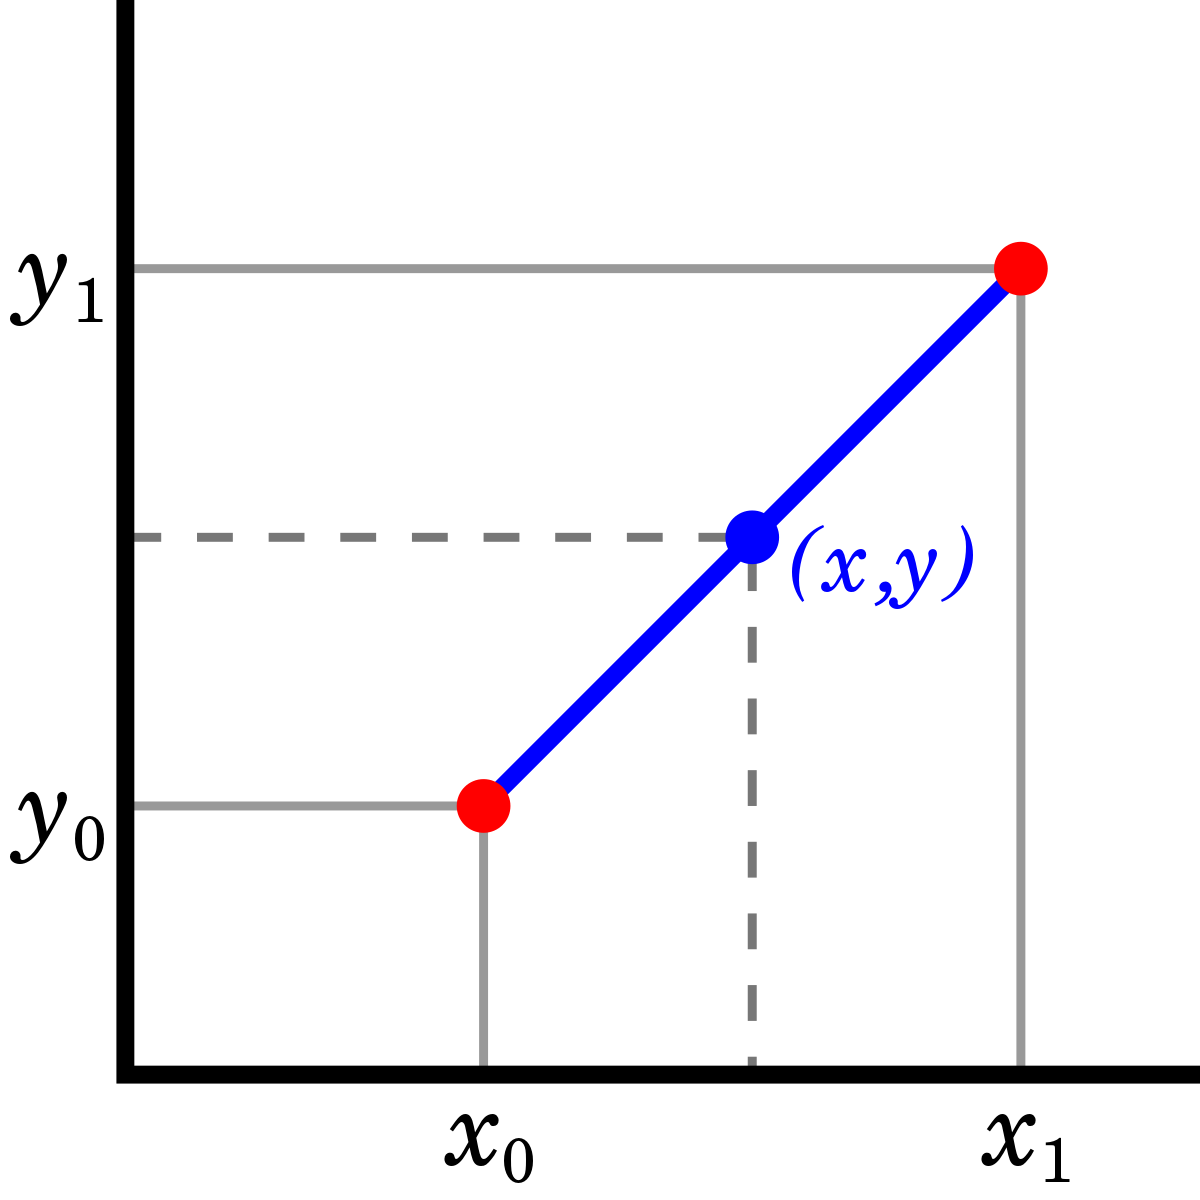
\includegraphics[width=0.5\textwidth]{images/interpolation.png}
    \end{figure}
    \end{multicols*}
\end{frame}

\begin{frame}
    \frametitle{Naivni pristop}
    \begin{itemize}
        \item Želimo si prilagodljivost in odgovornost
        \item Vsak član $S$ podpiše $(M, S) \rightarrow \sigma_i$
        \item Kot na papirju
        \item Primer: Ponudniki cen na omrežju Flare 
    \end{itemize}
    \vspace{1cm}
    Težava?
        $\sigma_1, \sigma_2, \sigma_3, \sigma_4, \sigma_5, \sigma_6,
        \sigma_7,  \sigma_8, \sigma_9, \sigma_{10}, \sigma_{11}, \sigma_{12}, 
        \sigma_{13}, \sigma_{14}, \sigma_{15}, \dots$
\end{frame}

\begin{frame}
    \frametitle{Skupni podpisi (angl. \textit{multisignatures})}
    \begin{itemize}
        \item Skupina vrne samo en podpis
        \item Prilagodljivost in odgovornost
        \item Naivna ideja + učinkovitost
        \item Primer: Podpisovanje peticij
    \end{itemize}
\end{frame}

\begin{frame}
    \frametitle{Schnorrov podpis}
    \framesubtitle{Generiranje ključev}
    \begin{itemize}
        \item $p, q \in \mathbb{P}$, $q\text{ }|\text{ }p-1$
        \item $g \in \mathbb{Z}_p^*$, $g^q \equiv 1 \pmod{p}$, torej $\text{ord}(g) = q$
        \item $s \in [0, q-1]$
        \item $I = g^s \bmod{p}$
    \end{itemize}
    \vspace{1cm}
    \begin{multicols*}{2}
        \textbf{Javni ključ}: $(p, q, g, I)$
        \columnbreak

        \textbf{Zasebni ključ}: $s$
    \end{multicols*}
\end{frame}

\begin{frame}
    \frametitle{Schnorrov podpis}
    \framesubtitle{Podpisovanje in preverjanje}
    \begin{itemize}
        \item Podpis sporočila $M$ je par $(X, y)$
        \item $r \in [0, q-1]$
        \item $X = g^r \bmod{p}$
        \item $e = H(X, M)$
        \item $y = es + r \bmod{q}$
    \end{itemize}
    
    \vspace{1cm}
    \begin{itemize}
        \item Preverimo, če je $(X', y')$ veljaven podpis za $M$
        \item $e' = H(X', M)$
        \item $g^{y'} \stackrel{?}{\equiv} X' \cdot I^{e'} \pmod{p}$
    \end{itemize}
\end{frame}

\begin{frame}
    \frametitle{Začetna ideja}
    \framesubtitle{Osnovni pojmi}
    \begin{itemize}
        \item Skupina $G = P_1, P_2, \dots, P_L$
        \item Podmnožica podpisnikov $S$ je znana vnaprej, poljubna
        \item Vsi v skupini imajo dostop do naključnega oraklja $H$
        \item Napadalec: 
            \begin{itemize}
                \item Ima dostop do $H$
                \item Kontrolira vse komunikacijske kanale
                \item Cilj: ponarediti podpis
            \end{itemize}
    \end{itemize}
\end{frame}

\begin{frame}
    \frametitle{Začetna ideja}
    \framesubtitle{Generiranje ključev}
    \begin{itemize}
        \item Vsi v skupini poznajo \alert{$p, q$} in \alert{$g$}
        \item Vsak podpisnik $P_i$: 
            \begin{align*}
                s_i &\in [0, q-1] \\
                I_i &= g^{s_i} \bmod{p}
            \end{align*}
    \end{itemize}
    \vspace{1cm}
    \begin{multicols*}{2}
        \textbf{Javni ključi}: $(\alert{p, q, g}, I_i)$
        \columnbreak

        \textbf{Zasebni ključi}: $s_i$
    \end{multicols*}
\end{frame}

\begin{frame}
    \frametitle{Začetna ideja}
    \framesubtitle{Podpisovanje}
    \begin{center}
        $r_i \in [0, q-1]$ \\
        $X_i = g^{r_i} \bmod{p}$ \\
        \vspace{0.25cm}
        $\downarrow$ \\
        \vspace{0.25cm}
        $\tilde{X} = \prod_{P_i \in S} X_i \bmod{p}$ \\
        \vspace{0.25cm}
        $\downarrow$ \\
        \vspace{0.25cm}
        $e = H(\tilde{X}, M, S)$ \\
        $y_i = e s_i + r_i \bmod{q}$ \\
        \vspace{0.25cm}
        $\downarrow$ \\
        \vspace{0.25cm}
        $\tilde{y} = \sum_{P_i \in S} y_i \bmod{q}$ \\
    \end{center}
\end{frame}

\begin{frame}
    \frametitle{Začetna ideja}
    \framesubtitle{Preverjanje}
    \begin{itemize}
        \item Preverimo, če je $(\tilde{X}', \tilde{y}')$ veljaven podpis za $M$
        \item $e' = H(\tilde{X}', M, S)$
        \item $g^{\tilde{y}'} \stackrel{?}{\equiv} \tilde{X}' \cdot (\prod_{P_i \in S} I_i)^{e'} \pmod{p}$   
    \end{itemize}
\end{frame}

\begin{frame}
    \frametitle{Problem 1}
    \framesubtitle{Skupni parametri}
    \begin{itemize}
        \item Kako generiramo $p, q, g$?
        \item Če si pomagamo z orakljem, to pozna tudi napadalec
        \vspace{1cm}
        \item \textbf{Rešitev}: Del DLP, varna praštevila
    \end{itemize}
\end{frame}

\begin{frame}
    \frametitle{Problem 2}
    \framesubtitle{$I_A = g^{s_A} \bmod p$}
    \begin{itemize}
        \item Napadalec goljufa pri izračunu $I_A$
        \item Lahko podpisuje v imenu skupine
        \vspace{1cm}
        \item \textbf{Rešitev}: Dokaz brez razkritja znanja, potrebno preverjanje 
                vsakega javnega ključa
    \end{itemize}
\end{frame}

\begin{frame}
    \frametitle{Dokazi brez razkritja znanja}
    \begin{itemize}
        \item Dokaz, da nekaj vemo, ne da bi razkrili kaj vemo
        \item Interaktivni protokol
    \end{itemize}
    \vspace{1cm}
    \begin{figure}
        \begin{subfigure}{0.32\textwidth}
            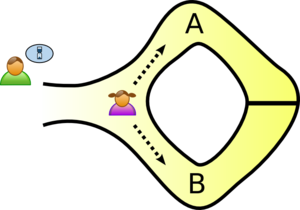
\includegraphics[width=\textwidth]{images/zkp1.png}
        \end{subfigure}
        \hspace{0.25cm}
        \begin{subfigure}{0.3\textwidth}
            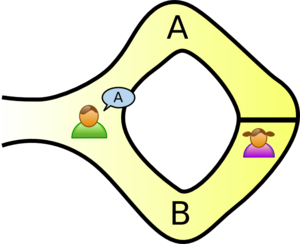
\includegraphics[width=\textwidth]{images/zkp2.png}
        \end{subfigure}
        \hspace{0.25cm}
        \begin{subfigure}{0.3\textwidth}
            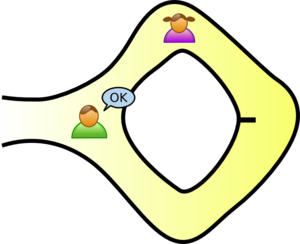
\includegraphics[width=\textwidth]{images/zkp3.png}
        \end{subfigure}
    \end{figure}
\end{frame}

\begin{frame}
    \frametitle{Fiat-Shamirjeva hevristika}
    \begin{itemize}
        \item Pretvorba interaktivnega dokaza v neinteraktivnega
        \item Interaktivnost zamenja naključni orakelj
        \item Če oraklji ne obstajajo, hevristika ni varna
    \end{itemize}
\end{frame}

\begin{frame}
    \frametitle{(Ne)interaktivni dokaz}
    \begin{itemize}
        \centering
        \item A: Poznam $x$, da $y \equiv g^x \bmod q$
        \item A: Naključni $v$, da $t \equiv g^v \bmod q$
        \item A: Pošlje $t$
    \end{itemize}
    \vspace{1cm}
    \begin{multicols*}{2}
        \begin{itemize}
            \item B: Naključni $c$, pošlje A
        \end{itemize}
        \begin{itemize}
            \item A: Izračuna $c = H(g, y, t)$
        \end{itemize}
    \end{multicols*}
    \vspace{1cm}
    \begin{itemize}
        \centering
        \item A: Pošlje $r = v - cx \bmod{\varphi(q)}$ B
        \item B: Preveri $t \stackrel{?}{\equiv} g^r y^c \bmod q$
    \end{itemize}
\end{frame}

\begin{frame}
    \frametitle{Problem 3}
    \framesubtitle{Preverjanje dokazov}
    \begin{itemize}
        \item Kdo preverja dokaze brez razkritja znanja?
        \vspace{1cm}
        \item \textbf{Rešitev}: Dokaz brez razkritja znanja del javnega ključa
    \end{itemize}
\end{frame}

\begin{frame}
    \frametitle{Problem 4}
    \framesubtitle{Velikost $S$}
    \begin{itemize}
        \item Število podpisnikov omejeno
        \item Tehnikalije v dokazu varnosti
        \vspace{1cm}
        \item \textbf{Rešitev}: Podpis $\sigma_i$ sporočila 
            $H(X_1, I_1, X_2, I_2, \dots, X_L, I_L)$
    \end{itemize}
\end{frame}

\begin{frame}
    \frametitle{Problem 5}
    \framesubtitle{Velikost ključa}
    \begin{itemize}
        \item V ključ moramo torej dati $\sigma_i$ in $X_1, I_1, X_2, I_2, 
        \dots X_L, I_L$
        \item Predolg ključ, proporcionalen velikosti $G$
        \vspace{1cm}
        \item \textbf{Rešitev}: Merklovo drevo z listi $I_1, I_2, \dots, I_L$
    \end{itemize}  
\end{frame}

\begin{frame}
    \frametitle{Merklova drevesa}
    \begin{figure}
        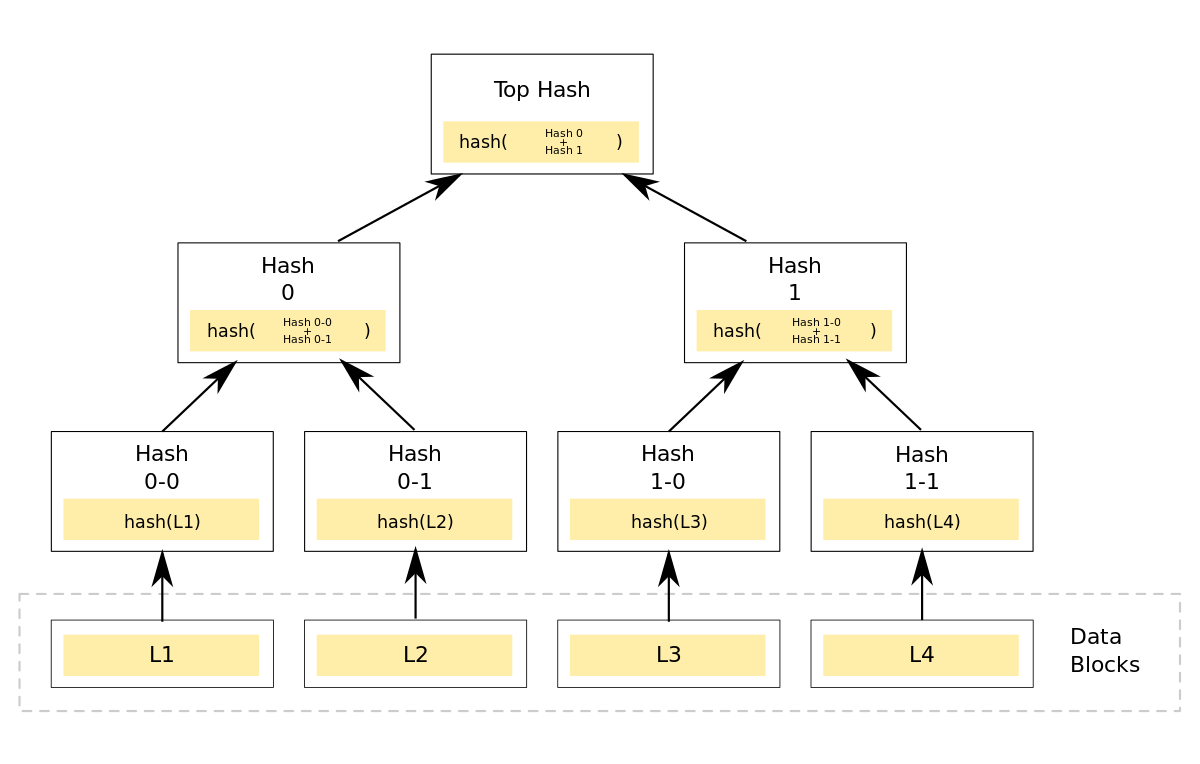
\includegraphics[width=\textwidth]{images/merkle-tree.png}
    \end{figure}
\end{frame}

\begin{frame}
    \frametitle{Problem 6}
    \framesubtitle{Sočasno podpisovanje}
    \begin{itemize}
        \item Dokaz varnosti uporablja previjanje (angl. \textit{rewinding})
        \vspace{1cm}
        \item \textbf{Rešitev}: Ne dovolimo sočasnega podpisovanja
    \end{itemize}
\end{frame}

\begin{frame}
    \frametitle{Končna shema}
\end{frame}

\begin{frame}
    \frametitle{Varnost}
\end{frame}

\end{document}